\documentclass[twoside,12pt,a4paper]{scrreprt}
\usepackage[T1]{fontenc}
\usepackage[utf8]{inputenc}
\usepackage[ngerman]{babel}
\usepackage{babelbib}
\usepackage{parskip}
\usepackage{microtype}
\usepackage{graphicx} % Zum Einbinden von Grafiken
\usepackage[dvipsnames]{xcolor}
\usepackage[colorlinks=true,linkcolor=Black,citecolor=MidnightBlue,urlcolor=MidnightBlue]{hyperref}
\usepackage[all]{hypcap}
\usepackage{pgfplots} \pgfplotsset{compat=1.9}
\usepackage{helvet} % Schönere SansSerif-Schrift
\usepackage{times}  % Schönere Serif-Schrift

\pagestyle{headings}

\graphicspath{ {figures/} } % Pfad-Prefix für einzubindende Grafiken. Es sind auch mehrere Pfade möglich, diese müssen jeweils in eigenen {Klammern} stehen.

\setkomafont{disposition}{\normalcolor\bfseries} % überall Serifen verwenden
% oder
%\renewcommand{\familydefault}{\sfdefault} % überall Sans-Serif verwenden

% PDF-Optionen (werden in den Dateieigenschaften angezeigt)
\hypersetup{
pdftitle={Implementierung und Evaluierung eines Additionsspiels über Partnerzahlen für Grundschüler},
pdfauthor={Marco Piechotta},
pdfsubject={Bachelorarbeit Informatik},
pdfpagelayout=TwoColumnRight
}

%%% Eigene Makros
\newcommand{\qq}[1]{\glqq #1\grqq} % \qq{Text in Anführungszeichen}

\begin{document}

%%% Titelseite
\begin{titlepage}
\begin{center}
\LARGE Eberhard Karls Universität Tübingen\\
\large Mathematisch-Naturwissenschaftliche Fakultät \\
Wilhelm-Schickard-Institut für Informatik\\
[3cm]
\huge Bachelorarbeit Informatik\\
[2cm]
\Large\textbf{Implementierung und Evaluierung eines Additionsspiels über Partnerzahlen für Grundschüler}\\
[1.5cm]
\large Marco Piechotta\\
[0.5cm]
\today
\\
\vfill
\small\textbf{Gutachter}\\[0.3cm]
\large Name Gutachter\\
\footnotesize Wilhelm-Schickard-Institut für Informatik\\Universität Tübingen\\
[1cm]

\small\textbf{Betreuer}\\[0.3cm]
\large Heiko Holz\\
\footnotesize Adresse\\
Universität Tübingen

\small\textbf{Betreuer}\\[0.3cm]
\large Manuel Ninaus\\
\footnotesize Leibniz-Institut für Wissensmedien\\
Schleichstraße 6
72076 Tübingen
\end{center}
\end{titlepage}

%%% Titelrückseite: Bibliographische Angaben
\thispagestyle{empty}
\vspace*{\fill}
\textbf{Piechotta, Marco:}\\
\emph{Implementierung und Evaluierung eines Additionsspiels über Partnerzahlen für Grundschüler}\\
Bachelorarbeit Informatik\\
Eberhard Karls Universität Tübingen\\
Bearbeitungszeitraum: 1. Oktober 2018 --- 31. Januar 2019
\newpage

%%% Zusammenfassung (Abstract), hier aus externer Datei eingebunden
\input{chapters/zusammenfassung.tex}
\newpage

%%% Inhaltsverzeichnis
\KOMAoption{toc}{listof,bib} % Abbildungs-/Tabellenverzeichnis, Literaturverzeichnis aufnehmen
\tableofcontents\label{toc}
\cleardoublepage

%%% Hauptteil (mit \input{dateiname} wird die Datei 'dateiname' eingebunden)
\input{chapters/einleitung.tex}
\cleardoublepage

% !TEX root = ../ausarbeitung.tex

\chapter{Stand der Forschung}
Hier zeigen Sie, dass Sie über Ihr Themengebiet gut informiert sind. Sie können entweder den Stand der Forschung dafür heranziehen, um Ihr Thema zu rechtfertigen (\qq{Warum ist es wichtig?}) oder Sie können die Literatur als Grundlage Ihrer Diskussion verwenden (Wie ordnen sich Ihre Beiträge in die Wissenschaftslandschaft allgemein ein?), eine Mischung ist auch möglich.

\hfil\rule{0.4\textwidth}{0.4pt}

Dazu gehören natürlich Referenzen zu anderen Werken. Für deren Verwaltung empfiehlt sich BibTeX, die entsprechende Datei \verb|literatur.bib| (kann natürlich auch anders benannt sein) ist in der Vorlage schon enthalten. Zur Einhaltung der Syntax bietet sich ein Online-Editor wie \cite{BibTexOnlineEditor} an; TeXstudio \cite{texstudio} hält im Menü auch Hilfe beim Erstellen der Bibliographie-Einträge bereit. Für Bücher bietet z.B. auch \url{https://books.google.de/} fertige BibTeX-Einträge an.

Die Einbindung in den Text erfolgt dann mit \verb|\cite{nielsen1994usability}|, wobei der Text in den Klammern durch das in der \verb|.bib|-Datei vergebene Kürzel ersetzt werden müssen. Das Ergebnis ist dann eine Referenz zum (zumindest im Bereich \qq{Usability Engineering}) fast unverzichtbaren gleichnamigen Buch \cite{nielsen1994usability} von Jakob Nielsen.

Achtung: Ihre Ausarbeitung sollte sich (im Gegensatz zu diesem Template) weniger auf Internet-Quellen, als auf Bücher und Paper stützen!
\\

\Blindtext[5]
\cleardoublepage

% !TEX root = ../ausarbeitung.tex
%%% DELETE THIS LATER
%Im Hauptteil beschreiben Sie Ihre praktische Arbeit. Code gehört %normalerweise nicht in eine Ausarbeitung. Ausnahmen sind Algorithmen, %die für Sie wichtig waren (dann in möglichst übersichtlichem Pseudo-%Code). Kleine Code-Stücke können auch zur Illustration oder als Beispiel %eingebaut werden. Längere Code-Stücke können im Anhang %untergebracht werden. Sie sollten jedoch nicht den gesamten Code im %Anhang abdrucken. Ihren Code geben Sie bitte dennoch mit ab, am %besten auf einer CD.
%
%Der Detailgrad sollte so sein, dass ein Leser die gleiche Arbeit noch %einmal nachimplementieren könnte. Insbesondere sollten alle Parameter, %von denen die Funktionsweise des Systems abhängt, explizit genannt %sein. Bei der Evaluation muss bei jedem Versuch angegeben werden, mit %welchen Parametern gearbeitet wird.
\chapter{Herangehensweise}
In diesem Kapitel wird der Weg von der Konzipierung mehrerer Konzepte für das Lernspiel bis zur Implementierung des Spiels behandelt.
\section{Konzeptwahl des Spiels}
\subsection{Erste Idee Math Smashers}
Die erste Idee ein Lernspiel zu entwickeln, welches Grundschüler unterstützt die Addition über das Konzept der Partnerzahlen zu erlernen, war das bereits vorhandene Spiel \textit{Math Smashers}\cite{ludoscience}.\\
In \textit{Math Smashers} fliegen Bälle mit Zahlen herum. Als Spieler kann man eine Art Seil als Verbindung zwischen zwei Kugeln anbringen. Dieses Seil zieht sich zusammen um die Kugeln zusammenzufassen (siehe \ref{fig:mathsmashers}) und deren Zahlen zu addieren (z.B. eine Kugel mit der Zahl 18 und eine mit der Zahl 4 gibt zusammengefasst eine Kugel mit der Zahl 22). Ziel ist es alle Bälle so zu addieren, damit man eine gesuchte Zahl (z.B. 22) heraus bekommt. Dabei kann es auch vorkommen mehrmals die gesuchte Zahl zu bekommen.
\begin{figure}[htb]
	\centering
	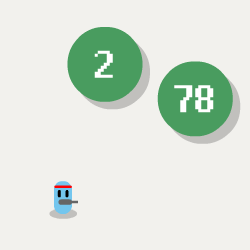
\includegraphics[width=0.3\textwidth]{MathSmasher-NotConnected}
	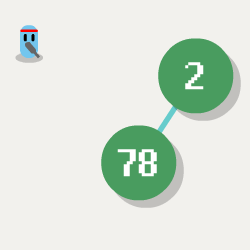
\includegraphics[width=0.3\textwidth]{MathSmasher-Connected}
	\caption{MathSmashers links zwei nicht verbundene Zahlen. Rechts beide Zahlen verbunden.\label{fig:mathsmashers}}
\end{figure}
\subsection{Weitere Ideenfindung}
Zunächst wurden weitere Ideen erarbeitet, wie das Konzept der Partnerzahlen noch in einem Spiel untergebracht werden kann. Dabei entstanden die folgenden vier Ideen.
\subsubsection{Kombination mit \qq{The Legend of Zelda}}
Diese Idee ist als Anlehnung an das Spiel \textit{The Legend of Zelda} gedacht. Kombiniert wird es mit dem bereits beschriebenen \textit{Math Smashers}. In diesem Fall werden, statt Bällen, die aus \textit{The Legend of Zelda: Majoras Mask}\cite{zelda} bekannten Schleimgegner, die Zahlen enthalten, verwendet. Ziel ist es auch hier zwei Zahlen zu einer Gesuchten zu addieren, indem Schleimgegner mit den passenden Partnerzahlen besiegt und die im Schleim liegenden Zahlen addiert.
\begin{figure}[htb]
	\centering
	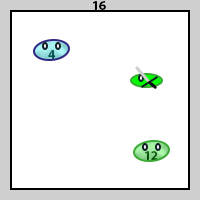
\includegraphics[width=0.45\textwidth]{Zelda-Skizze}
	\caption{Skizze der Legend of Zelda Idee\label{fig:zelda}}
\end{figure}
\subsubsection{Murmeladdierer}
Diese Idee überträgt das Vorhaben auf ein altes Murmelspiel. Es gibt mehrere Löcher, die mit Zahlen beschriftet sind, in welche die Kugeln hinein manövriert werden müssen. Die Bewegung der Kugeln wird durch das Kippen des Spielfelds in eine bestimmte Richtung erzielt. Wie in jedem der vorgestellten Ansätze wird hier eine gesuchte Zahl bereitgestellt. Da zwei Kugeln gleichzeitig auf dem Feld zu bewegen sehr schwer sein könnte, kann man das ganze auch sequenziell mit jeweils einer Kugel spielen.
\begin{figure}[htb]
	\centering
	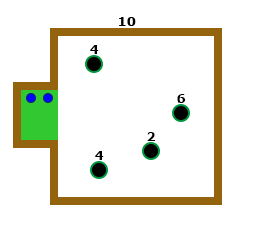
\includegraphics[width=0.3\textwidth]{HolesImg}
	\caption{Skizze des Murmeladdierer Spiels\label{fig:murmadd}}
\end{figure}
\subsubsection{Zahlenbausteine}
Auch für diese Idee ist es wieder nötig Zahlen zu einer gesuchten Zahl zu addieren. Hier sind die Zahlen in Form von Ziegelsteinen gegeben und der Spieler muss ein Gebäude errichten, welches mehrere dieser Ziegelsteine benötigt. Diese sind mit den gesuchten Zahlen beschriftet. Der Spieler muss sich zwei Steine auf dem Spielfeld suchen und diese aufeinander legen um sie zum gesuchten Ziegelstein zu addieren. Dieser muss anschließend vom Spieler an die richtige Position im Bauwerk gebracht werden.
\begin{figure}[htb]
	\centering
	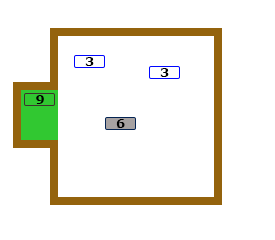
\includegraphics[width=0.4\textwidth]{BaukloetzeImg}
	\caption{Skizze des Zahlenbaustein Spiels\label{fig:baustein}}
\end{figure}
\subsubsection{MathSnake}
Für diese Idee wird das Addieren von Partnerzahlen zu einer gesuchten Zahl auf Snake übertragen. In diesem Snake gibt es Zahlenäpfel. Frisst die Schlange einen dieser Äpfel hat sie einen Teil der Partnerzahl gefressen und zur Addition hinzugefügt. Frisst sie den nächsten Apfel werden beide Zahlen addiert. Die Schlange wird pro Apfel länger und schneller.
\begin{figure}[htb]
	\centering
	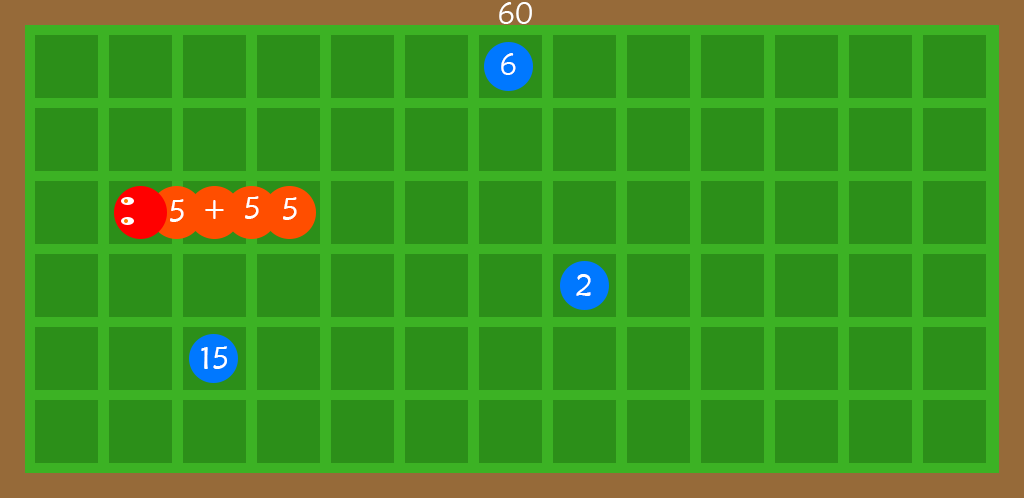
\includegraphics[width=0.49\textwidth]{Snake-Skizze}
	\caption{Skizze des MathSnake Spiels\label{fig:mathsnake}}
\end{figure}
\section{Wahl des Spielkonzepts und Entwicklung des Spiels}
Aus den erarbeiteten Konzepten habe ich mich für MathSnake entschieden, da diese Idee einem klassischen Spiel einen neuen Reiz verleiht. Die Kombination mit \textit{The Legend of Zelda} würde dies ebenfalls erfüllen, allerdings würde eine Umsetzung hier erheblich mehr Zeit in Anspruch nehmen, welche dann für die Evaluation gefehlt hätte. Außerdem bietet die MathSnake Variante mehr Möglichkeiten, das Spiel herausfordernder zu gestalten. Zum Beispiel durch Anstieg der Bewegungsgeschwindigkeit nach dem Essen eines Apfels und die Längenzunahme der Schlange. Aber auch durch weitere Features, wie dem Verfaulen der Äpfel über eine gewisse Zeit, lässt sich das Spiel schwieriger gestalten. Diese Aspekte waren ausschlaggebend um sich für die Snake Variante zu entscheiden.
MathSnake wurde in der Entwicklungsumgebung Unity umgesetzt, da diese sehr Einsteigerfreundlich ist und man bereits in kurzer Zeit gute Ergebnisse erzielen kann. Als Zielplatftorm wurde Android gewählt, um das Spiel auf einem bereitgestellten Tablet spielen zu können. Damit das Spiel möglichst professionell und kinderfreundlich aussieht, wurde sich für ein Asset-Pack aus dem Unity Asset Store entschiden. Durch dieses gab es bereits Grafiken für die Schlange und Gestaltungsdetails für die Umgebung. Die Umgebung selbst wurde in Blender modeliert und in Unity mit den gegebenen Details geschmückt.
\subsection{Verschiedene Spielversionen}
Im Zuge dieser Bachelorarbeit wurden zwei verschiedene Varianten umgesetzt und evaluiert. Zur Auswahl standen folgende Versionen mit deren erwarteten Vor- und Nachteilen.\\
\\
Dabei handelt es sich bei der TopDown-Perspektive um die Ansicht aus der Vogelperspektive auf das Spielgeschehen. Das heißt von oben mit Blick senkrecht nach unten. Während bei der Third-Person-Perspektive die Kamera direkt hinter dem Schlangenkopf positioniert wird. Die Unterschiede lassen sich in Abbildung \ref{fig:mathsnake-perspektives} erkennen.

\subsubsection{3D Snake mit Third-Person-Perspektive}
\begin{table}[h!]
\centering
\begin{tabular}{|l|l|}
\hline
\multicolumn{1}{|c|}{\textbf{Vorteile}}                                                                         & \multicolumn{1}{c|}{\textbf{Nachteile}}                                                                               \\ \hline
modern                                                                                                        & \begin{tabular}[c]{@{}l@{}}wenig Übersicht über das Spielfeld, welche Zahlen wo\\ liegen ist nicht gegeben\end{tabular} \\ \hline
\begin{tabular}[c]{@{}l@{}}mehr das Gefühl als Spieler\\ die Schlange zu sein.\end{tabular}                     &                                                                                                                       \\ \hline
\begin{tabular}[c]{@{}l@{}}Spielfeld kann abwechslungsreich\\ über mehrere Ebenen gestaltet werden\end{tabular} &                                                                                                                 \\ \hline
\begin{tabular}[c]{@{}l@{}}Übersicht auf welcher Ebene man sich\\ befindet ist sehr gut\end{tabular}            &  \\ \hline
\begin{tabular}[c]{@{}l@{}}wenig Übersicht kommt dem Such-\\ charakter allerdings zugute.\end{tabular}          &  \\ \hline
\end{tabular}
\caption{Gegenüberstellung von Vor- und Nachteilen der Variante 3D Snake mit Third-Person-Perspektive\label{fig:3dthird}}
\end{table}
\subsubsection{3D Snake mit TopDown-Perspektive}
\begin{table}[h!]
\centering
\begin{tabular}{|l|l|}
\hline
\multicolumn{1}{|c|}{\textbf{Vorteile}} & \multicolumn{1}{c|}{\textbf{Nachteile}}                                                                 \\ \hline
modern                                  & \begin{tabular}[c]{@{}l@{}}Schlechte Übersicht darüber, auf welcher\\ Ebene man sich bewegt\end{tabular} \\ \hline
mehrere Spielfeldebenen möglich         &                                                                                                         \\ \hline
Gute Übersicht wo welche Zahl liegt     &                                                                                                         \\ \hline
                                        &                                                                                                         \\ \hline
                                        &                                                                                                         \\ \hline
\end{tabular}
\caption{Gegenüberstellung von Vor- und Nachteilen der Variante 3D Snake mit TopDown-Perspektive\label{fig:3dTop}}
\end{table}
\subsubsection{2D Snake mit TopDown-Perspektive}
\begin{table}[h!]
\centering
\begin{tabular}{|l|l|}
\hline
\multicolumn{1}{|c|}{\textbf{Vorteile}} & \multicolumn{1}{c|}{\textbf{Nachteile}}                                                                         \\ \hline
einfache Umsetzung                      & kein neuer Anreiz gegenüber dem klassischen Snake                                                                                                    \\ \hline
Grafisch nicht so aufwändig             & \begin{tabular}[c]{@{}l@{}}weniger Möglichkeiten den Spieler\\ über Level-Elemente herauszufordern\end{tabular} \\ \hline
Gute Übersicht wo welche Zahl liegt     &                                                                                                                 \\ \hline
                                        &                                                                                                                 \\ \hline
                                        &                                                                                                                 \\ \hline
\end{tabular}
\caption{Gegenüberstellung von Vor- und Nachteilen der Variante 2D Snake mit TopDown-Perspektive\label{fig:2dTop}}
\end{table}
\subsection{Grid-Spielfeld}
Weiterhin stand zur Auswahl ob das SnakeSpiel mit oder ohne einem Grid-Spielfeld erstellt werden soll. Unter einem Grid-Spielfeld wird ein Spielfeld verstanden, dass in einzelne kleinere Felder aufgeteilt ist, auf denen sich die Schlange bewegen kann. Pro 'Zug' bewegt sich die Schlange jeweils ein Feld weiter und füllt dieses Feld komplett aus.
\subsubsection{Snake mit Grid}
\begin{table}[h!]
\centering
\begin{tabular}{|l|l|}
\hline
\multicolumn{1}{|c|}{\textbf{Vorteile}}                                                     & \multicolumn{1}{c|}{\textbf{Nachteile}}                                                      \\ \hline
einfache Steuerung                                                                          & \begin{tabular}[c]{@{}l@{}}weniger Freiheiten für den Spieler\\ sich zu bewegen\end{tabular} \\ \hline
\begin{tabular}[c]{@{}l@{}}einfach um neue Objekte in die\\ Spielwelt zu legen\end{tabular} & weniger Freiheiten im Leveldesign                                                            \\ \hline
\begin{tabular}[c]{@{}l@{}}Objekte können nicht ineinander\\ liegen\end{tabular}            &                                                                                              \\ \hline
                                                                                            &                                                                                              \\ \hline
                                                                                            &                                                                                              \\ \hline
\end{tabular}
\caption{Gegenüberstellung von Vor- und Nachteilen des Snake-Spiels mit einem Grid-Spielfeld\label{fig:grid}}
\end{table}
\subsubsection{Snake ohne Grid}
\begin{table}[h!]
\centering
\begin{tabular}{|l|l|}
\hline
\multicolumn{1}{|c|}{\textbf{Vorteile}}                                                                 & \multicolumn{1}{c|}{\textbf{Nachteile}} \\ \hline
moderne Steuerung                                                                                       & Objekte können ineinander liegen        \\ \hline
\begin{tabular}[c]{@{}l@{}}Spieler kann sich in mehr als\\ vier Richtungen bewegen\end{tabular}            & Aufwändiger in der Umsetzung            \\ \hline
\begin{tabular}[c]{@{}l@{}}Leveldesign kann durch verschiedene\\ Formen unterstützt werden\end{tabular} &                                         \\ \hline
                                                                                                        &                                         \\ \hline
                                                                                                        &                                         \\ \hline
\end{tabular}
\caption{Gegenüberstellung von Vor- und Nachteilen des Snake-Spiels ohne einem Grid-Spielfeld\label{fig:nogrid}}
\end{table}
Entschieden wurde sich für die beiden 3D Varianten ohne Grid, da das Ziel ist, beide Versionen vergleichen zu können um zu ermitteln, welche Version bei Spielern besser ankommt. Ein großer Vorteil, die beiden 3D Varianten zu implementieren, ist auch, dass so nur die Perspektive geändert werden kann ohne die Grafiken neu anpassen zu müssen. So blieb der Fokus auf der unterschiedlichen Perspektive auf das Spielgeschehen. Um eine moderne Steuerung zu ermöglichen, habe ich mich außerdem gegen ein Spielfeld mit Grid entschieden. 
\section{Aufbau und Funktionsweise des Spiels}
\subsection{Aufbau des Spiels}
\subsubsection{Menüführung}
Der Aufbau des Spiels ist einfach gehalten. Der Spieler beginnt das Spiel im Hauptmenü, welches in Abbildung \ref{fig:mathsnake-menu}, in Form eines Ablaufplans, dargestellt wird. In diesem kann er sich für eine Spielversion entscheiden, die Highscore Tabelle begutachten oder das Spiel beenden. Startet er eine der beiden Spielversionen beginnt direkt das Spiel. 
\begin{figure}[htb]
	\centering
	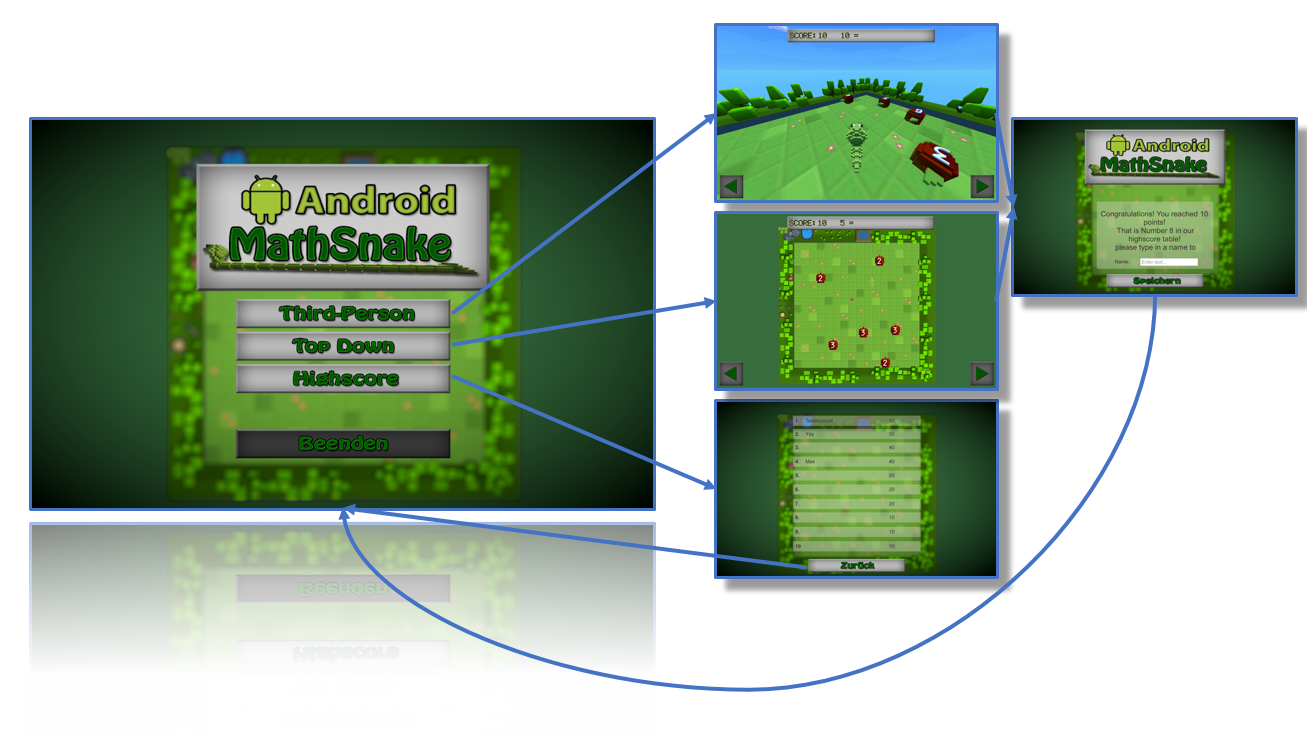
\includegraphics[width=0.85\textwidth]{MathSnake-Overview}
	\caption{Hauptmenü von MathSnake\label{fig:mathsnake-menu}}
\end{figure}
\subsubsection{Spielfeldaufbau}
Der Spieler sieht am oberen Bildschirmrand die gesuchte Zahl gefolgt von einem '=' ( Beispielsweise ' 5 = ' ). Auf dieses folgen dann alle gefressenen Zahlen mit einem '+' verbunden ( z.B. 5 = 1 + 1 + 3 ). Dies stellt die Gleichung dar, die erfüllt sein muss, um die Aufgabe zu bestehen. Links neben der gesuchten Zahl findet der Spieler auch seinen aktuellen Score. Dieser nimmt bei einer falschen Zahl ab und bei einer richtigen Zahl zu. Der Spieler kann die Schlange über zwei Pfeiltasten steuern. Diese zwei Tasten geben die Richtung an, in die sich die Schlange bewegen soll. Der Spieler kann sie über diese Tasten nach rechts oder links bewegen. Die einzelnen Felder werden auch nochmals in der Abbildung \ref{fig:mathsnake-setup} verdeutlicht.
\begin{figure}[htb]
	\centering
	\includegraphics[width=0.75\textwidth]{MathSnake-setup}
	\caption{Ansicht auf den Aufbau des Spiels\label{fig:mathsnake-setup}}
\end{figure}
\subsubsection{Highscore}
Das Spiel stellt auch eine simple Highscore Liste bereit, um einen weiteren Anreiz zu schaffen. Diese wird für den Nutzertest deaktiviert, da die Nutzer sich voll auf die Bewertung des Spiels an sich konzentrieren sollen und der Highscore nicht Teil der Forschungsfragen ist.\\
Ist der Highscore aktiviert, wird dem Spieler nach dem Ende einer Spielrunde eine Nachricht angezeigt. Dem Spieler wird in dieser angezeigt, ob er genügend Punkte gesammelt hat, um sich in der Highscore Liste einzutragen. Dies geschieht dann über ein Textfeld in dessen er seinen Name eingeben kann, wie in Abbildung \ref{fig:mathsnake-newHighscore} zu sehen ist.
\begin{figure}[htb]
	\centering
	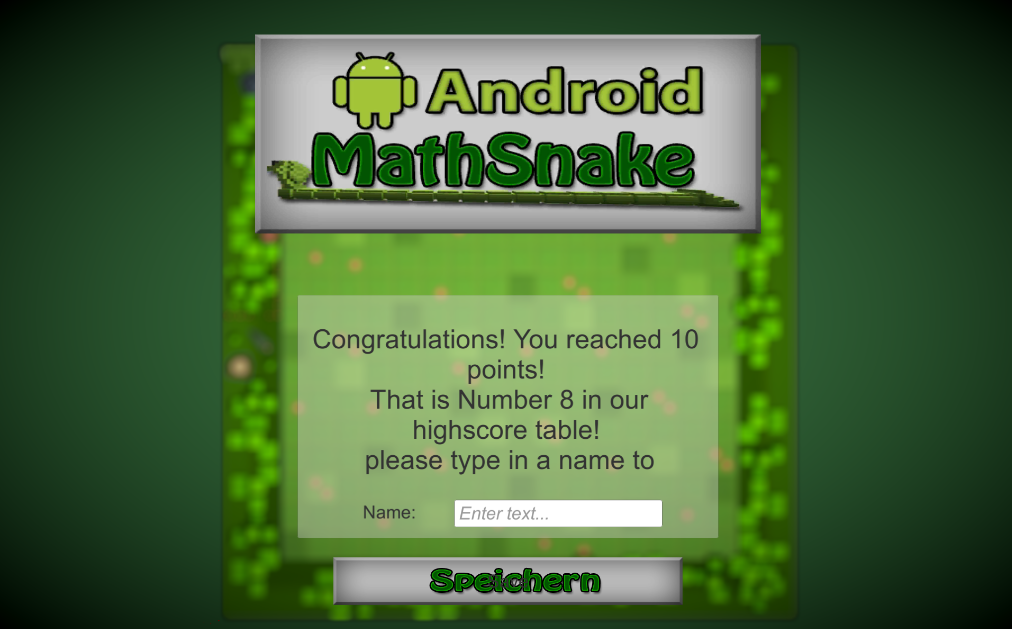
\includegraphics[width=0.65\textwidth]{MathSnake-Highscore1}
	\caption{Erstellen eines neuen Highscore-Eintrags\label{fig:mathsnake-newHighscore}}
\end{figure}
Im Hauptmenü kann, wie in Abbildung \ref{fig:mathsnake-menu} zu erkennen ist, die aktuelle Highscore-Tabelle angezeigt werden. Diese ist so aufgebaut, dass Platz 1 mit der höchsten Punktzahl oben steht. Gibt es Spieler mit der gleichen Punktzahl schlägt ein neueres Ergebnis ein Älteres. In Abbildung \ref{fig:mathsnake-HighscoreTable} ist eine beispielhafte Ansicht der Highscore-Tabelle abgebildet.
\begin{figure}[htb]
	\centering
	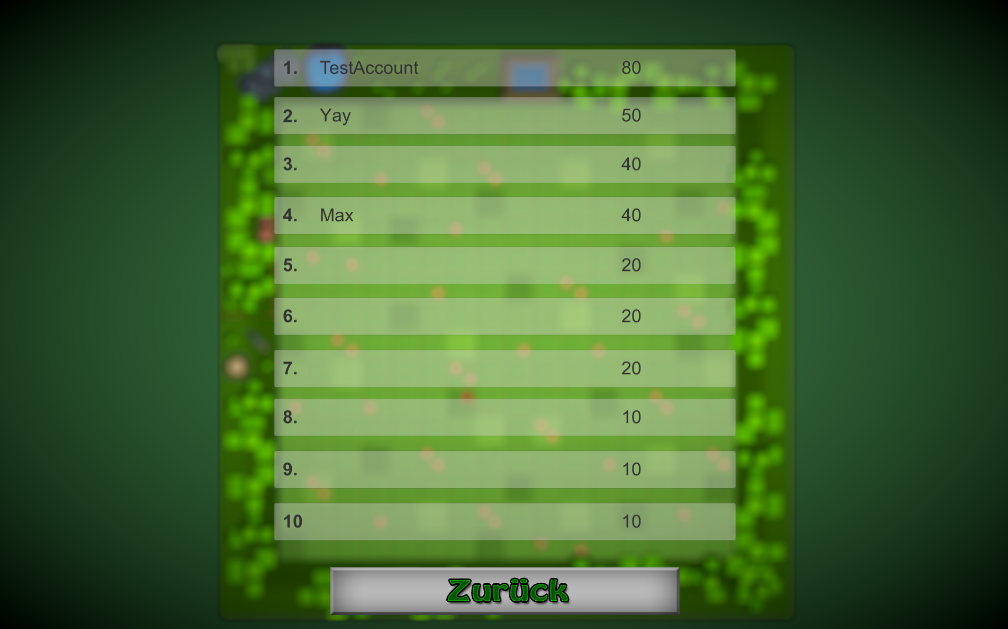
\includegraphics[width=0.65\textwidth]{MathSnake-Highscore2}
	\caption{Ansicht der Highscore-Tabelle\label{fig:mathsnake-HighscoreTable}}
\end{figure}
\subsection{Funktionsweise des Spiels}
Das entwickelte Spiel lässt sich nun entweder in der TopDown Ansicht oder in der Third-Person Ansicht spielen. Die Funktionsweise bleibt bei beiden identisch. Der Spieler steuert eine Schlange und kann diese mit zwei Pfeiltasten nach rechts oder links drehen, um die Bewegungsrichtung zu verändern. Am oberen Bildschirmrand wird ihm eine gesuchte Zahl, sowie seine aktuelle Punktzahl, angezeigt. Hat die Schlange einen Apfel mit einer Zahl gefressen wird diese durch ein + getrennt dem Gleichtungsbereich(siehe \ref{fig:mathsnake-setup}) hinzugefügt. Mit jedem gegessenem Apfel wird die Schlange schneller und länger.
\begin{figure}[htb]
	\centering
	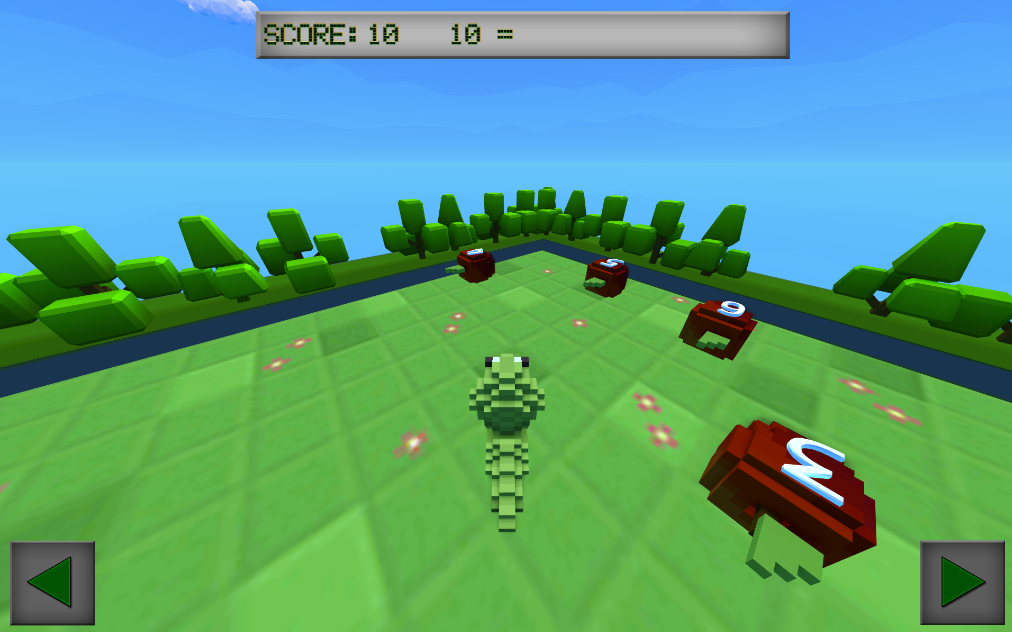
\includegraphics[width=0.35\textwidth]{MathSnake-ThirdPerson}
	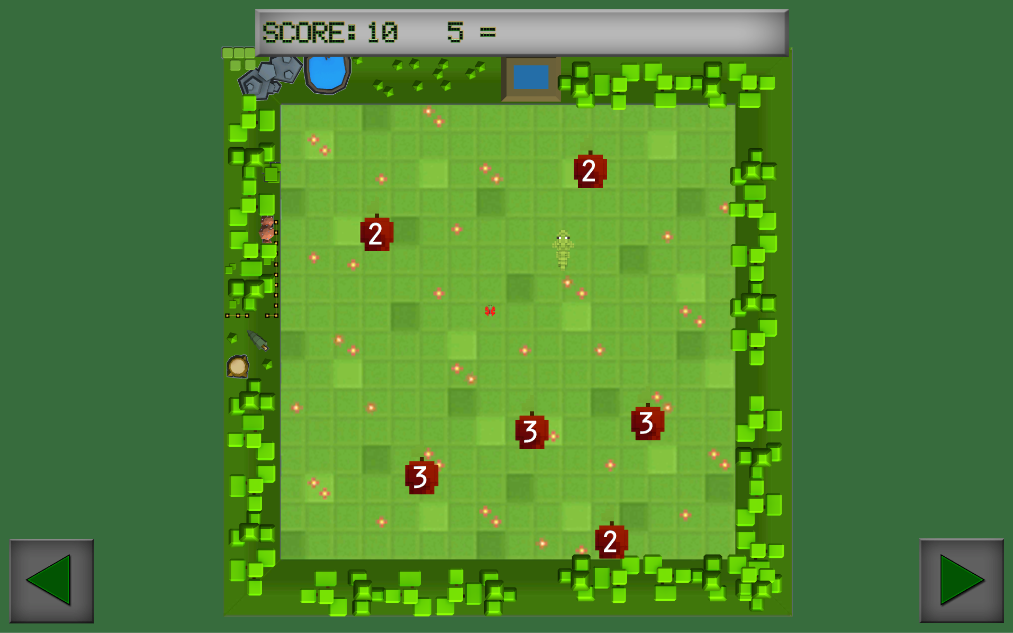
\includegraphics[width=0.35\textwidth]{MathSnake-TopDown}
	\caption{Links: Third-Person und Rechts: TopDown Perspektive\label{fig:mathsnake-perspektives}}
\end{figure}
\subsubsection{Levelsystem}
Pro zu suchender Zahl gibt es ein Level. Um das Spiel auf Dauer herausfordernder zu gestalten, wurde ein kleines Levelsystem eingeführt. Dabei varriiert der Zahlenraum je nachdem in welchem Levelbereich der Spieler sich befindet. Im höchsten Bereich beginnen die Äpfel zu verfaulen. Die implementierte Zuordnung ist der Tabelle \ref{tab:levels} zu entnehmen.
\begin{table}[h!]
\centering
\begin{tabular}{|l|l|l|}
\hline
\textbf{Level} & \textbf{Zahlenbereich} & \textbf{Eigenschaften}       \\ \hline
0-4            & 3-20                   & -                            \\ \hline
5-9            & 20-50                  & -                            \\ \hline
10-19          & 50-100                 & -                            \\ \hline
20-49          & 30-100                 & -                            \\ \hline
50+            & 30-100                 & Äpfel verfaulen mit der Zeit \\ \hline
\end{tabular}
\caption{Bedeutung der einzelnen Levelbereiche\label{tab:levels}}
\end{table}

\cleardoublepage

% !TEX root = ../ausarbeitung.tex
%Erklärung des Nutzertests mit Testgruppe, was herausgefunden werden soll:
%A: Macht so ein Spiel für Partnerzahlen Spaß?
%B: Welche Version ist besser?
\chapter{Evaluation} %TODO Ref
Im Rahmen dieser Arbeit wurde versucht über den GEQ zwei Fragen zu beantworten. Zunächst sollte überprüft werden ob dieses Additionsspiel zur Unterstützung des Lernprozesses bei Addition über Partnerzahlen den Kindern Spaß bereitet. Außerdem sollte ermittelt werden welche der beiden implementierten Versionen besser bei den Kindern ankommt. Zur Beantwortung wurde der GEQ Fragebogen abgewandelt zur KidsGEQ Variante damit Grundschüler alle Fragen verstehen und beantworten können.
\section{Game Experience Questionnaire}
Der Game Experience Questionaire wurde 2013 an der Universität für Technologie in Eindhoven definiert \cite{IJsselsteijn2013}.
Beim normalen GEQ werden 3 Module eingebaut:
\begin{itemize}
\item Core questionaire
\item Social Presence Module
\item Post-game Module
\end{itemize}
Diese Module werden direkt nach einer Spielrunde durchgegangen, dabei testen die ersten beiden Module wie der Spieler sich beim spielen gefühlt hat, während das Post-Game Module testet wie der Spieler sich nach dem beenden des spielens gefühlt hat.
\subsection{Core questionaire}
In diesem Teil werden dem Spieler Fragen aus den Kategorien Challenge, Competence, Flow, Immersion, Negative Effect, Positive Effect und Tension gestellt. Um eine gute Messung zu erzielen und Puffer zu haben um wenn nötig Fragen streichen zu können, sollte man 5 Fragen pro Kategorie verwenden. In der Auswertung sollte hier außerdem die Gewichtung der Fragen überprüft werden, da es sein kann das bei der Ausführung mit einer Frage Probleme auftreten können. Wenn sie zum Beispiel nicht verstanden wurde, kann es sein das man diese Frage aus der Auswertung entfernen muss.
\subsubsection{Challenge}
Mit den Challenge Fragen wird beim GEQ der Schwierigkeitsgrad des Spiels ermittelt. Der Schwierigkeitsgrad des Spiels kann durch mehrere Faktoren beeinflusst werden. Zum einen kann die Aufgabe einfach schwer gewählt sein, aber auch durch die technische Umsetzung und dem Design kann der Schwierigkeitsgrad angehoben werden. Auf diesen Einfluss wird in der Diskussion noch weiter eingegangen.
\subsubsection{Competence}
In der Competence Kategorie sollen Fragen beantwortet werden, die darauf abzielen ob das Spiel intuitiv ist. Das heißt der Spieler sollte zu jeder Zeit wissen, was seine Aufgabe ist und wie er der Erfüllung dieses Ziels näher kommt.
\subsubsection{Flow}
Der Flow-Wert beschreibt wie stark das Spiel die Aufmerksamkeit des Spielers eingenommen hat und wie 'vertieft'  er in das Spiel war.
\subsubsection{Immersion}
In dieser Kategorie soll geprüft werden, wie die Ästhetik des Spiels ist. Dies betrifft sowohl ob das Spiel Visuell überzeugen konnte, als auch ob man durch das Spiel die Fantasie des Spielers anregen konnte.
\subsubsection{Negative Effect}
Hier soll über Fragen ermittelt werden, ob das Spiel negative Einflüsse auf den Spieler hat. Diese Einflüsse können dazu führen, dass das Spiel dem Spieler keinen Spaß bereitet. Bei bestimmten Genres, wie Horrorspielen, können negative Einflüsse, wie Angst, allerdings auch gewollt sein. Im Fall von MathSnake sollten diese aber möglichst minimiert werden.
\subsubsection{Positive Effect}
Unter dieser Kategorie versteht man Fragen, die ermitteln sollen ob das Spiel positive Einflüsse auf den Spieler hatte. Diese führen dazu, dass sich der Spieler durch das Spiel besser fühlt, da er zum Beispiel lachen musste.
\subsubsection{Tension}
In dieser Kategorie zielen die Fragen auf die Gemütslage des Spielers ab. Hier können Erkenntnisse darüber gewonnen werden ob das Spiel noch zu unausgereift ist. Dies ist dann der Fall, wenn der Spieler sich über das Spiel mehrfach beschwert, da er weiß wie er sein Ziel erreichen kann, aber zum Beispiel die Steuerung ist zu sensibel oder verzögert.
\subsubsection{Bestimmung der Kategoriewerte}
Um den Wert jeder Kategorie für einen Teilnehmer des Nutzertests zu bestimmen, werden die Antwortmöglichkeiten von 0 bis 4 gewichtet. Anschließend addiert man nach dieser Skala alle Werte der jeweiligen Kategorie auf und teilt ihn durch die Anzahl an Fragen. 
\subsection{Social Presence Module} %TODO Ref!
Das Social Presence Module wird benötigt um die psychologische und verhaltensbezogene Einbindung des Spielers ins Spielgeschehen zu messen. Dies geschieht entweder virtuel, durch In-Game Characteren mit denen Gesprochen werden kann so genannten NPC's, mediated, wenn das Spiel einen Online-Modus besitzt, oder co-located. Das Modul sollte nur dann eingesetzt werden, wenn mindestends eines dieser Einbindungen des Spielers vorhanden sind.
\subsection{Post-Game Module}
Das Post-Game Module wird verwendet um zu prüfen wie sich die Spieler nach dem Ende der Spielphase fühlen. Dieses Modul ist besonders deswegen relevant, da man hier ermitteln kann ob der Spieler zum Beispiel freiwillig spielen möchte oder eigentlich keine Lust mehr auf das Spiel hat.
\section{Umsetzung des KidsGEQ}
In der umgesetzten Version wurden pro Kategorie 3 Aussagen gewählt, die zunächst ins deutsche übersetzt wurden und anschließend in möglichst leicht für Kinder verständliche Sprache umformuliert. Diese 21 Aussagen sollen nun von den Kindern anhand einer Skala beantwortet werden. Diese Skala ist in 5 Kategorien aufgebaut: 'überhaupt nicht', 'ein wenig', 'mittel', 'ziemlich', 'sehr'. Die Frage an die Kinder ist wie stark sie der jeweiligen Aussage zustimmen. Der Grad der Zustimmung wird zusätzlich durch einen Farbcode hervorgehoben. 

\begin{figure}[htb]
	\centering
	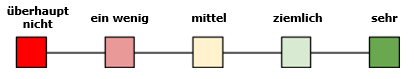
\includegraphics[width=0.75\textwidth]{farbskala}
	\caption{Farbskala der einzelnen Fragen\label{fig:farbskala}}
\end{figure}

Außerdem wurde eine weitere Frage mit dieser Skala hinzugefügt um abzufragen wie gut die Kinder mit der Steuerung zurecht gekommen sind. Abschließend zu diesen 22 Ankreuzfragen gab es noch 3 schriftliche Fragen um am Ende eine klare Antwort auf die Forschungsfragen zu forcieren. %TODO richtig mit forciert?
\section{Durchführung des Nutzertests} %TODO Zufällige Version?
Der Nutzertest wurde in 2 Phasen durchgeführt. Zunächst durften die Kinder eine Version für 10 Minuten spielen. Anschließend gab es den ersten Fragebogen mit den 22 Fragen. Nach einer kurzen Pause von ca. 5 Minuten in denen sich mit etwas komplett anderem beschäftigt wurde, ging es zu den zweiten 10 Minuten spielen der anderen Version. Nach dieser Spielzeit wurde wieder der Fragebogen ausgefüllt mit den abschließenden 3 schriftlichen Fragen. Insgesamt ergab dies eine Versuchsdauer von ca. 30 Minuten pro Person.\\
\\
Der Nutzertest wurde mit einer kleinen Anzahl an Kindern durchgeführt aufgrund dessen, dass in der Weihnachtszeit nur sehr schwer Testpersonen im Alter der Zielgruppe gefunden werden kann. Die Menge an Testpersonen umfasste 5 Grundschulkinder aus den ersten Klassenstufen. Diese kleine Menge lässt zwar keine statistischen Erhebungen zu, allerdings können wir darauf deskriptive Statistik anwenden. 

\hfil\rule{0.4\textwidth}{0.4pt}
\cleardoublepage

% !TEX root = ../ausarbeitung.tex
%Unter Evaluation der Result Teil mit "nackten Zahlen" als Boxplot + Textuell %Mittelwert und Standardabweichung. Wenn möglich noch ein statistischen Test %zwischen den einzelnen Kategorien.
\chapter{Results} %TODO Ref
In diesem Kapitel werden die Ergebnisse des Nutzertests präsentiert. Die Darstellung erfolgt nach den Kategorien, die durch den GEQ definiert wurden. Anhand von Boxplots werden die Ergebnisse der jeweiligen Kategorie von der ThirdPerson Ansicht und der TopDown Ansicht gegenüber gestellt.
Zunächst wird ein Gesamtbild der beiden Perspektiven, für einen groben Überblick, gegenüber gestellt.
\begin{figure}[h!tb]
	\centering
	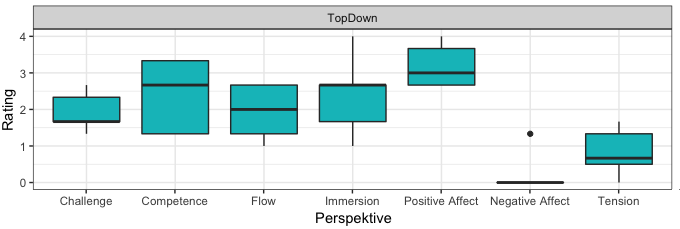
\includegraphics[width=0.65\textwidth]{topDownPlot}
	\caption{Boxplots der TopDown Perspektive\label{fig:topdownbox}}
\end{figure}
\begin{figure}[h!tb]
	\centering
	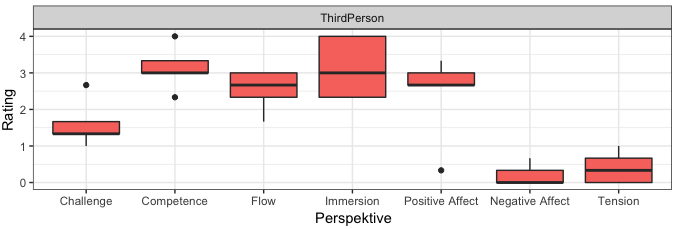
\includegraphics[width=0.65\textwidth]{thirdPersonPlot}
	\caption{Boxplots der ThirdPerson Perspektive\label{fig:thirdpersonbox}}
\end{figure}
\section{Challenge}
\begin{figure}[h!tb]
	\centering
	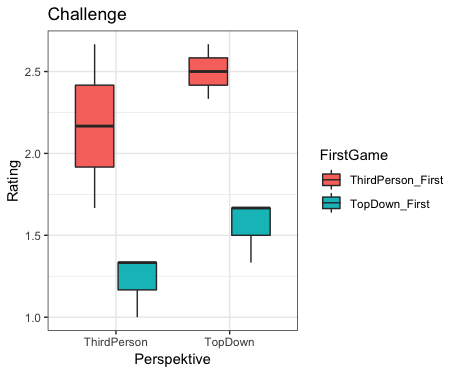
\includegraphics[width=0.65\textwidth]{challengePlot}
	\caption{Boxplot der Kategorie Challenge\label{fig:challengebox}}
\end{figure}
Der Durchschnitt in der Challenge Kategorie beträgt für TopDown zuerst $1.8\overline{8}$
\section{Competence}
\begin{figure}[h!tb]
	\centering
	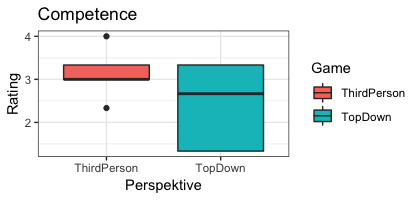
\includegraphics[width=0.65\textwidth]{competencePlot}
	\caption{Boxplot der Kategorie Competence\label{fig:competencebox}}
\end{figure}

\section{Flow}
\begin{figure}[h!tb]
	\centering
	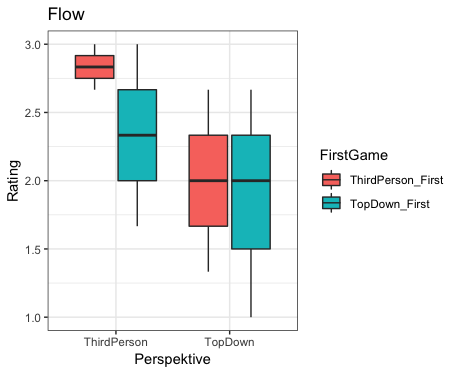
\includegraphics[width=0.65\textwidth]{flowPlot}
	\caption{Boxplot der Kategorie Flow\label{fig:flowbox}}
\end{figure}

\section{Immersion}
\begin{figure}[h!tb]
	\centering
	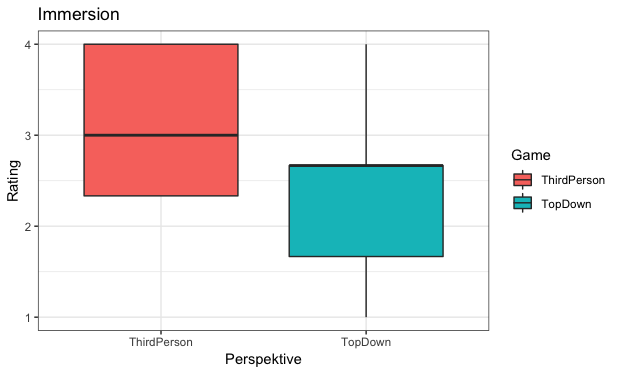
\includegraphics[width=0.65\textwidth]{immersionPlot}
	\caption{Boxplot der Kategorie Immersion\label{fig:immersionbox}}
\end{figure}

\section{Negative Effect}
\begin{figure}[h!tb]
	\centering
	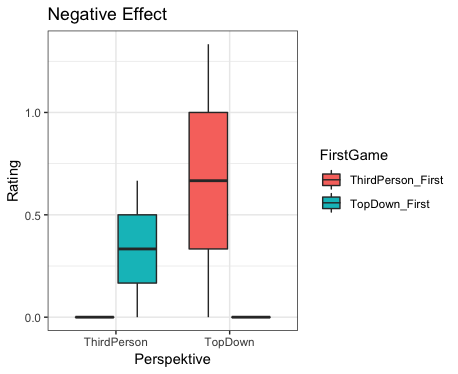
\includegraphics[width=0.65\textwidth]{negEffPlot}
	\caption{Boxplot der Kategorie Negative Effect\label{fig:negeffbox}}
\end{figure}

\section{Positive Effect}
\begin{figure}[htb]
	\centering
	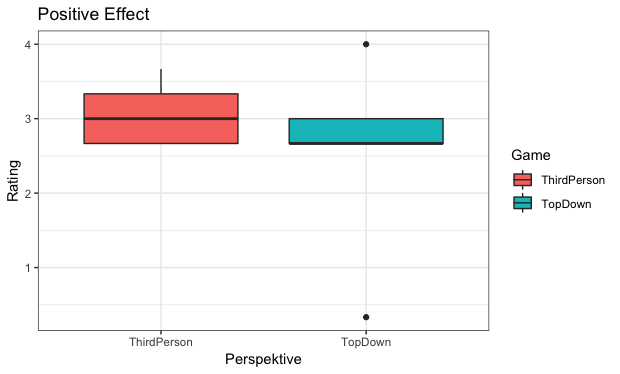
\includegraphics[width=0.65\textwidth]{posEffPlot}
	\caption{Boxplot der Kategorie Positive Effect\label{fig:poseffbox}}
\end{figure}

\section{Tension}
\begin{figure}[htb]
	\centering
	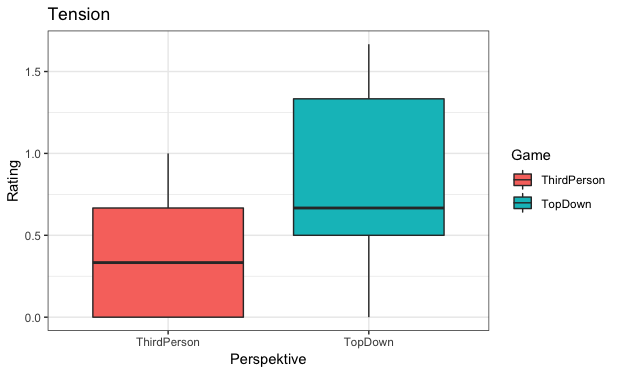
\includegraphics[width=0.65\textwidth]{tensionPlot}
	\caption{Boxplot der Kategorie Tension\label{fig:tensionbox}}
\end{figure}

\hfil\rule{0.4\textwidth}{0.4pt}
\cleardoublepage

% !TEX root = ../ausarbeitung.tex

\chapter{Diskussion} %TODO Ref!!!
\label{chap:discussion}
In diesem Kapitel sollen die Ergebnisse des Nutzertests interpretiert werden. Generell lässt sich erkennen, dass die Nutzer Spaß an beiden Spielversionen hatten. Die Ergebnisse legen aber nah, dass das Spiel mit der Third-Person-Perspektive den Kindern besser gefallen hat. Dies wird durch die Folgenden Unterkapitel der einzelnen Kategorien näher begründet.
\section{Challenge}
\label{sec:challengeDisk}
Der Durchschnitt der Challengebewertungen in der TopDown Perspektive liegt höher als in der ThirdPerson Perspektive. Dies könnte daran liegen, da es in der TopDown Perspektive schwieriger war die Schlange zu erkennen, da die Schlange und der Boden eine ähnliche Farbe haben. In der ThirdPerson Perspektive war die Schlange leichter erkennbar, da die Kamera sehr nah an der Schlange war. Durch diese Perspektive musste man teilweise nicht die grüne Farbe der Schlange von der grünen Farbe der Umgebung unterscheiden, da der Himmel in dieser Perspektive auch sichtbar war. Einen Vergleich hierzu sieht man in Abbildung \ref{fig:mathsnake-perspektives}.

\section{Competence}
\label{sec:competenceDisk}
In dieser Kategorie wurde abgefragt, wie erfolgreich sich die Spieler während des Spielens gefühlt haben. Hier fällt auf, dass es in der TopDown Ansicht größere Schwankungen gibt. Auf diesen Wert kann der Kontrast der Schlange einen Einfluss genommen haben, da sich die Spieler weniger erfolgreich fühlten wenn sie die Schlange nicht genau erkennen konnten. Der Median liegt hier aber im oberen Bereich. Dies kann daran liegen, dass Spieler, die zuerst die Third-Person-Perspektive gespielt haben einen leichteren Umstieg auf die TopDown Version hatten. Das Spielprinzip war zu dieser Zeit bereits klar, sowie welche Art von Charakter man im Spiel steuert. Es ist jedoch zu erwähnen, dass die Third-Person-Perspektive bessere Tendenzen zeigt, da hier die Competence-Werte enger beieinander liegen.
\section{Flow}
\label{sec:flowDisk}
Hier ist zu erkennen, dass tendenziell die ThirdPerson Perspektive den Spieler mehr eingenommen hat. Dies kann darin begründet sein, dass in dieser Perspektive der Spieler eher das Sichtfeld des zu steuernden Charakters sieht als in der TopDown-Perspektive. Ein weiterer Grund hierfür kann sein, dass der Spieler sich hier mehr auf das Spiel konzentrieren muss, da er nicht direkt alle Zahlen im Überblick hat. In der TopDown-Perspektive sieht der Spieler direkt alle Äpfel, mit deren Zahlen, und kann sich leicht einen Plan zurecht legen. In der Third-Person-Perspektive sieht dies anders aus. Hier muss sich der Spieler erst einen Überblick über das Spielfeld verschaffen, um ein Apfelpaar zu finden, welches addiert die gesuchte Zahl ergibt. Dies wird außerdem dadurch erschwert, dass die Zahlen sich nicht zum Spieler drehen und damit nicht immer optimal angezeigt werden. Der Spieler muss also auch umgedrehte Zahlen lesen können. Dies alles deutet darauf hin, dass der Spieler sich in der ThirdPerson Variante mehr auf das Spiel fokusieren muss. 
\section{Immersion}
\label{sec:immersionDisk}
Auch der Immersions-Wert der ThirdPerson Variante deuted darauf hin, dass diese Version den Spielern besser gefallen hat. Dies kann dadurch begründet sein, dass der Spieler in der TopDown Perspektive schnell alles gesehen hat, während man in der ThirdPerson Perspektive die Umgebung erst erkunden kann und mehr Details der Umgebung sehen kann als in der TopDown Perspektive.
\section{Positive Effect} %TODO vielleicht noch etwas schreiben?
\label{sec:poseffDisk}
Die Werte für die Positiven Effekte während des Spielens sind für beide Versionen sher ähnlich mit um die 2.6 bis 3.5. Beide Versionen weisen aber die Tendenz auf, eher viele positive Effekte herforgerufen zu haben.
\section{Negative Affect}
\label{sec:negeffDisk}
In dieser Kategorie zeigen beide Spiele eher die Tendenz zu keine negativen Emotionen ausgelöst zu haben. Der Durchschnitt dieser Kategorie-Werte liegt für diese Stichprobe unter eins. Aus diesem Grund lässt sich sagen, dass sowohl die TopDown, als auch die Third-Person Version, des Spiels von den Kindern nicht als negativ wahrgenommen werden.
\section{Tension}
\label{sec:tensionDisk}
In dieser Kategorie hat sich vor allem während des Nutzertests die Frage 18 als interessant heraus gestellt.
\begin{quote}
\qq{Ich habe beim Spielen gemotzt}
\end{quote}
Der Boxplot zeigt uns hier, dass man im Schnitt in der TopDown Variante mehr Probleme hatte. Dies kann wieder, wie bereits in Unterkapitel \ref{sec:challengeDisk} erwähnt, daran liegen, dass die Schlange nicht gut erkennbar war. Hier waren die Kinder nicht mit der Steuerung zufrieden. Wenn die Schlange im TopDown Modus sich von unten nach oben bewegt, ist es ganz klar, dass beim drücken auf die rechte Pfeiltaste sich die Schlange nach rechts bewegt und beim drücken auf die linke Pfeiltaste sich die Schlange nach links bewegt. Dies trifft allerdings nicht mehr zu, wenn die Schlange sich von oben nach unten bewegt. Dieser Umstand hat den meisten Kindern Probleme bereitet und wird in Abbildung \ref{fig:controlIssue} nochmals grafisch dargestellt. Wenn die Pfeiltaste nach rechts durchgehend gedrückt gehalten wird, würde man zunächst das linke Bild sehen und anschließend das rechte Bild. Im klassischen Snake ist gibt es die vier Richtungstasten, die angeben in welche Richtung man sich bewegen möchte. Da ich mich für eine moderne Steuerung entschieden habe, mit der man sich frei über das Spielfeld bewegen kann, gab es hier die Möglichkeit für die vier Richtungstasten Steuerung nicht.
\begin{figure}[htb]
	\centering
	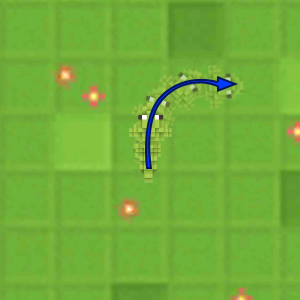
\includegraphics[width=0.3\textwidth]{SnakeDirection1}
	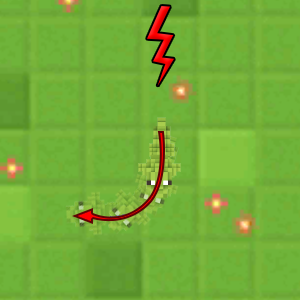
\includegraphics[width=0.3\textwidth]{SnakeDirection2}
	\caption{Links: Pfeiltaste nach rechts = nach rechts bewegen. Rechts: Pfeiltaste nach rechts = nach links bewegen\label{fig:controlIssue}}
\end{figure}
\section{Startpunktzahl}
\label{sec:startpointsDisk}
Am Anfang hatte jeder Spieler direkt 10 Punkte ohne einen Apfel gegessen zu haben, dies hätte eigentlich nicht der Fall sein sollen, hat aber weitere Beobachtungen eingebracht. Viele der Kinder scheinen nicht bemerkt zu haben, dass sie direkt mit 10 Punkten starten und gingen davon aus, dass sie schon etwas geschafft haben. Wenn die Kinder direkt am Anfang die Schlange sich selbst fressen ließen, fühlten siesich trotzdem ermutigt, da sie zumindest 10 Punkte erreicht hatten.
\section{Zusammenfassung und Ausblick}
\label{sec:ausblickDisk}
In diesem Kapitel soll die Arbeit nochmals zusammengefasst werden und die Erweiterungsmöglichkeiten des Spiels, sowie mögliche weitere Studien diskutiert werden.\\
\\
Insgesamt wurde die Zielsetzung dieser Arbeit, ein Mathelernspiel, zum erlernen der Addition, zu entwicklen, erfüllt. Das Spiel wurde in der Entwicklungsumgebung von Unity entwickelt, die als Einsteiger gut erlernbar ist. Damit konnte ich ein, durch den anschließenden Nutzertest bestätigtes, tolles Mathespiel entwickeln. Evaluiert wurde das Spiel über den Kids-GEQ Nutzertest. Dieser ermöglichte mir es einzelne Kategorien gezielt auszuwerten und auf die Forschungsfragen eine Antwort zu bekommen. Da das Spiel mit für das Tablet entwickelt wurde, konnte ich das Spiel leicht mit den fünf Kindern testen. Durch diese Arbeit konnte ich zeichen, dass die beide Versionen den Kindern gefallen, aber sie die Third-Person Version bevorzugen. Dies wurde zusätzlich, zu den vom Kids-GEQ gesammelten Daten, auch von den schriftlichen Fragen am Ende des Nutzertests bestätigt. Alle Nutzer haben bei der Frage, welches Spiel ihnen mehr Spaß gemacht hat die Third-Person Variante angegeben. Als schwieriger wurde von vier der fünf Kinder die TopDown Variante genannt. Diese Schwierigkeiten hatten vor allem Auswirkungen auf das Flow- und Challenge-Ergebnis, wie bereits in den Kapiteln \ref{sec:flowDisk} und \ref{sec:challengeDisk} beschrieben wurde.\\
Insgesamt können beide Forschungsfragen, aufgrund der geringen Stichprobenmenge, nicht eindeutig beantwortet werden. Allerdings kann anhand der Tendenzen gesagt werden, dass ein solches Lernspiel zur Unterstützung der Addition über Partnerzahlen den Kindern mit hoher Wahrscheinlichkeit Spaß bereitet. Außerdem konnte eine starke Tendenz zur Third-Person Variante erkannt werden. Ob diese nach Behebung einiger Schwierigkeiten der TopDown-Perspektive bestehen bleibt, ist durch zukünftige Tests zu ermitteln. Auch die generelle Wirksamkeit des Spiels ist durch weitere Nutzertests zu untersuchen.\\
\\
Das Spiel MathSnake lässt sich noch in vielen Bereichen verbessern. Eine Verbesserung im Design und den visuellen Effekten wäre, für die Third-Person Version den Kamerafehler am Ende einer Spielrunde zu entfernen. Es wäre hier interessant zu sehen ob das verzerrte Bild am Ende der Spielrunde negative Einflüsse auf das Spielgefühl bewirkt. Ein weiterer wichtiger Punkte ist, für die TopDown Version der Kontrast der Schlange. Dieser wurde mehrheitlich unter den Nutzern als verbesserungswürdig eingestuft. Da in dem verwendeten Asset-Pack mehrere Schlangendesigns enthalten sind, könnte der Spieler hier am Anfang des Spiels seine Schlange wählen. Dies könnte den Effekt haben, dass der Spieler sich auch gleichzeitig mehr mit seiner Spielfigur identifizieren kann und somit die wahrgenommene Autonomie, ein wichtiger Aspekt intrinischer Motivation\cite{Deci2000TheW}, addressiert werden könnte. Für einen vielleicht steigenden Immersions-Wert könnte zusätzlich sorgen, wenn die Grafik für den Boden überarbeitet werden, damit diese ebenso scharf dargestellt wird wie der Rest der Spielwelt.\\
\\
Auch für einen höheren Challenge-Wert kann das Spiel optimiert werden. So wäre es zum Beispiel möglich, das Spiel auch für höhere Klassenstufen interessanter zu gestalten. Der Anstieg der Schwierigkeitsstufe auf ein Level mit verfaulenden Äpfeln wurde für diesen Nutzertest so weit nach oben gesetzt, dass kein Spieler dieses Level erreichte. Das war für diese Altersgruppe aber auch nicht vorgesehen. In neueren Versionen kann also das Levelsystem angepasst werden, um auch zu diesem Level, nach einer angemessenen Spielzeit zu kommen. Auch mögliche Erweiterungen des Levelsystems wurden festgehalten. So ist es möglich weitere Level einzufügen in denen zum Beispiel 'Fake-Äpfel' auftauchen. Dies sind Äpfel, die dem Spieler effektiv nicht helfen die gesuchte Zahl zu bilden. Das heißt sie sollten von der Schlange nicht gegessen werden. Damit sind auch weitere Erweiterungen möglich, die die Schlange fressen kann. So ist es dann auch möglich ein Item einzuführen, welches diese 'Fake-Äpfel' identifizieren kann oder andere Eigenschaften mit sich bringt, wie Items die die Schlange verkürzen oder verlangsamen, aber auch Items mit denen der Spieler die zu suchende Zahl ändern kann als eine Art Joker.\\
\\
Es wäre auch interessant nicht nur die Addition zu untersuchen, sondern auch andere mathematische Operatoren. So könnte durch das einfache Hinzufügen von \qq{Operator-Äpfeln} die Komplexität und damit ebenfalls der Challenge-Faktor deutlich erhöht werden. Mit diesen speziellen Äpfeln wäre es außerdem möglich die Aufgabe an den Spieler zu varriieren. So kann er in einem Level ganz normal die Partnerzahlen suchen und in einem anderen sind die Zahlen der Gleichung vielleicht schon gegeben und er muss nur die richtigen Operatoren der Reihe nach einfügen. Im Gleichungsbereich könnte so etwas stehen wie $10 = 10   10   10$ und der Spieler bekommt Äpfel für die Multiplikation und Division.\\
\\
Auch für den Nutzertest sind Verbesserungen möglich. Indem eine größeren Stichprobenmenge verwendet wird, aber auch weitere Fragen können durch Nutzertests beantwortet werden. So zum Beispiel, ob Startpunkte, wie in Unterkapitel\ref{sec:startpointsDisk} beschrieben, den Wert der positiven Effekte steigert oder unerheblich für diesen ist. Außerdem wurde, wie in Unterkapitel \ref{sec:tensionDisk} beschrieben, ein Problem mit der Steuerung der TopDown Variante festgestellt. Hier ist über Nutzertests zu überprüfen, ob eine Änderung der Steuerung zur klassischen Snake Variante sinnvoll wäre. Im klassischen Snake steuert der Spieler die Schlange mit allen Richtungstasten und gibt jeweils an, in welche Richtung sich die Schlange bewegen soll. Dabei sind ausschließlich $90^\circ$ Drehungen möglich.

%TODO schönen Schluss schreiben wenn noch Zeit
\cleardoublepage

%%% Literaturverzeichnis, lädt die Datei literatur.bib
\bibliographystyle{babplain} % "babplain" benötigt das Paket babelbib
\bibliography{Bachelorthesis}
\cleardoublepage

%%% Selbständigkeitserklärung
\thispagestyle{empty}
\section*{Erklärung}
Hiermit erkläre ich, dass ich diese schriftliche Abschlussarbeit selbständig 
verfasst habe, keine anderen als die angegebenen Hilfsmittel und Quellen benutzt 
habe und alle wörtlich oder sinngemäß aus anderen Werken übernommenen Aussagen als 
solche gekennzeichnet habe.
\\[2cm]
Ort, Datum \hfil Unterschrift 

\end{document}